% Déclaration du type de document (report, book, paper, etc...)
\documentclass[a4paper]{report} 
 
% Package pour avoir Latex en français
\usepackage[utf8]{inputenc}
\usepackage[frenchb]{babel}
 
% Quelques packages utiles
\usepackage{listings} % Pour afficher des listings de programmes
\usepackage{graphicx} % Pour afficher des figures
\usepackage{amsthm}   % Pour créer des théorèmes et des définitions
\usepackage{amsmath}
\usepackage{microtype} % Optical margins FTW
\usepackage{url}
\usepackage{booktabs} % Allows the use of \toprule, \midrule and \bottomrule in tables for horizontal lines
\usepackage{siunitx}
\usepackage{floatrow}
\usepackage{caption}
\usepackage{subcaption}

% Début du document
\begin{document}

\begin{titlepage}

\newcommand{\HRule}{\rule{\linewidth}{0.5mm}} % Defines a new command for the horizontal lines, change thickness here

\center % Center everything on the page 
%----------------------------------------------------------------------------------------
%	HEADING 
%----------------------------------------------------------------------------------------
\textsc{\LARGE École Polytechnique Fédérale de~Lausanne}\\[1.5cm] 
\textsc{\Large Méthodes de Production}\\[0.5cm] % Major heading such as course name

%----------------------------------------------------------------------------------------
%	TITLE 
%----------------------------------------------------------------------------------------
\HRule \\[0.4cm]
{ \huge \bfseries Molded Interconnect Devices}\\[0.4cm] % Title of your document
\HRule \\[1.5cm]
 
%----------------------------------------------------------------------------------------
% LOGO EPFL
%----------------------------------------------------------------------------------------
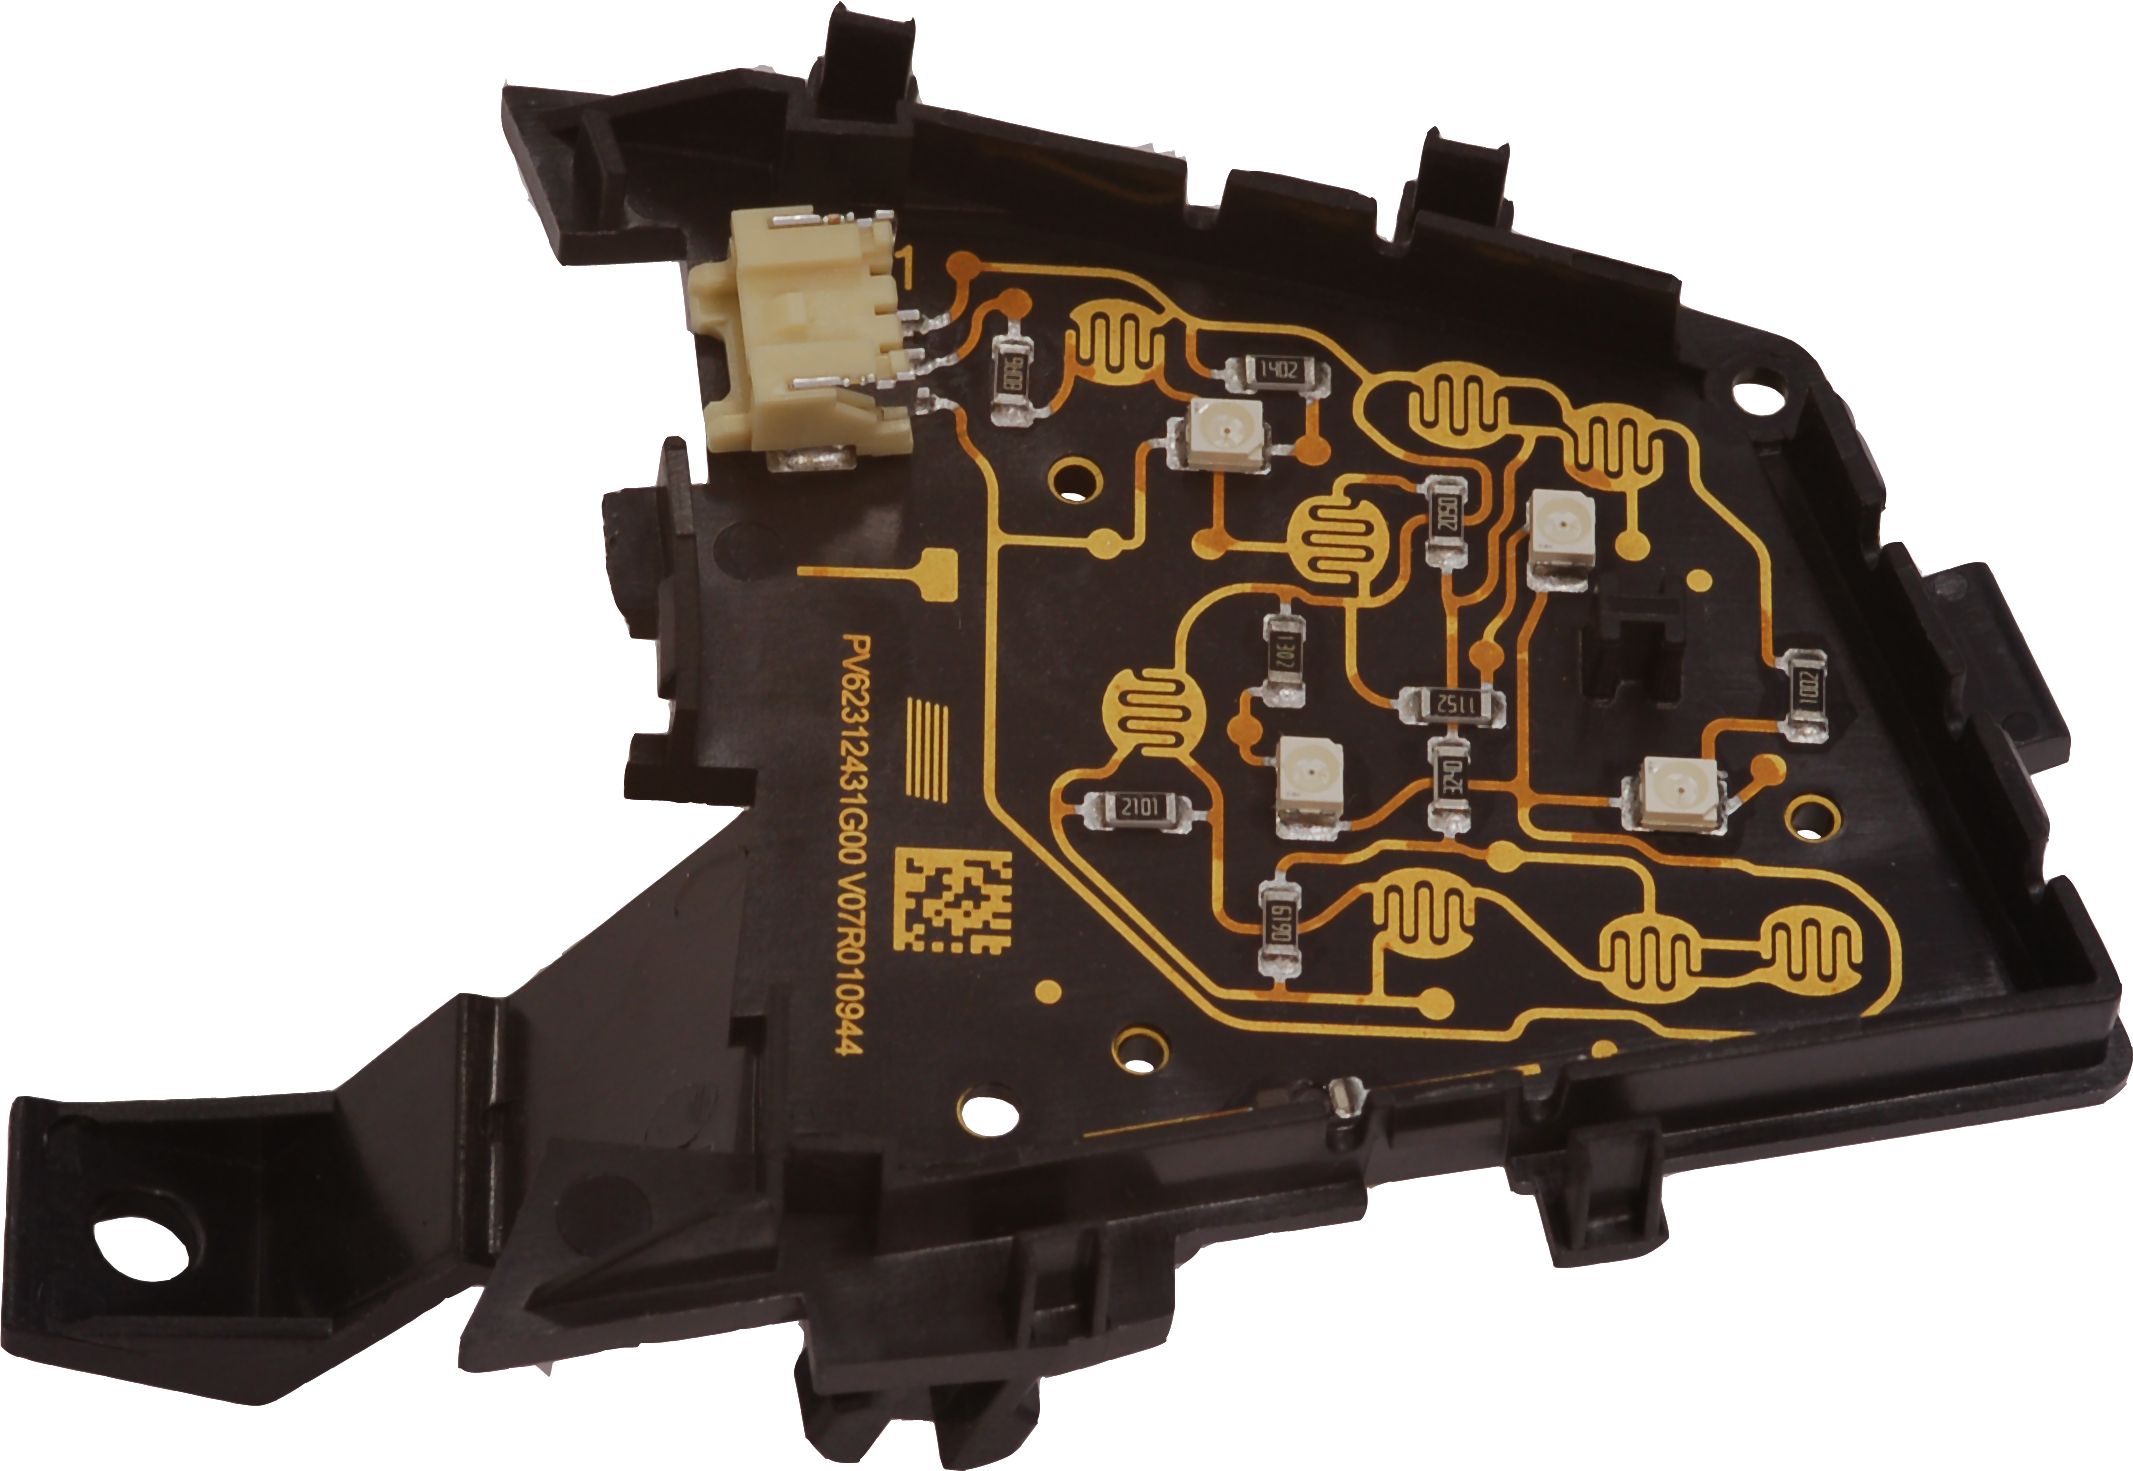
\includegraphics[width=0.8\textwidth]{../images/mid_example}\\[2cm]

%----------------------------------------------------------------------------------------
%	AUTHORS 
%----------------------------------------------------------------------------------------

\vfill % Fill the rest of the page with whitespace
\begin{minipage}{0.55\textwidth}
\begin{flushleft} \large
\emph{Étudiants:}\\
Antoine \textsc{Albertelli}\\ 
Quentin \textsc{Herzig}
\end{flushleft}
\end{minipage}
~
\begin{minipage}{0.4\textwidth}
\begin{flushleft} \large
\emph{Enseignants:} \\
Pr. Jacques \textsc{Jacot} \\
Pr. Peter \textsc{Ryser}\\
Dr. Jean-Daniel \textsc{Lüthi}
\end{flushleft}
\end{minipage}\\[2cm]


{\large 13 décembre 2013}
\end{titlepage}

% Empty page after title page.
\begin{titlepage}
    ~
\end{titlepage}



\tableofcontents

\clearpage
\section{Introduction}
Un \gls{mid}  est un circuit électronique
dont le support est un substrat thermoplastique moulé par injection, par
opposition au \textsc{PCB} conventionnels dont le substrat est un composite
plat.

Les \gls{mid} permettent de regrouper dans une seule pièce des fonctions
mécaniques et éléctroniques. En effet, contrairement au \textsc{pcb} conventionnels, les
\gls{mid} peuvent être conçus en trois dimensions, ce qui réduit
considérablement le nombre de composants et de connecteurs, diminuant ainsi le
temps d'assemblage, et donc le coût du système. 

Les \gls{mid}s ne sont toutefois pas une solution de remplacement des
\textsc{pcb}s car ils ne permettent pas une grande densité de pistes, tandis que
les \textsc{pcb}s à plus de deux couches sont désormais peu coûteux et
permettent des circuits à forte densité.


\section{Conception de MID}
La conception des \gls{mid} commence par la création du schéma électrique dans un logiciel de conception électronique standard, puis le schéma est exporté sous forme de \emph{netlist}, c'est à dire d'une liste de connexion entre différents composants.
Le design mécanique du \gls{mid} se fait dans un logiciel de \textsc{dao} standard, comme Solidworks puis est exporté au format \textsc{step}.

La \emph{netlist} et le fichier \textsc{step} sont ensuite importés dans un logiciel spécifique \footnote{Nextra de chez Mecadtron \url{http://www.mecadtron.com/produkte/nextra.en.php}} pour l'étape de routage (placement des pistes).
Lors de cette étape on place aussi des repères appelés \emph{fiducials} qui seront utilisés par les machines d'activation et d'assemblage pour faire un alignement visuel.
On peut également placer des codes-barres 2D (\emph{datamatrix}) qui seront modifiés par la machine d'activation pour y placer un numéro de série, afin de faire du suivi des pièces.

\subsection{Matériaux utilisables}
Les contraintes inhérentes à la technologie \gls{lds} limitent fortement le choix des matériaux :
\begin{itemize}
    \item La pièce étant injectée puis activée, le matériaux choisi doit être un thermoplastique,
    \item Pour l'étape d'activation, le polymère doit pouvoir se lier avec un dopant organométallique, généralement à base de palladium,
    \item L'assemblage des composants par \textit{reflow soldering} exige une température de fusion élevée.
\end{itemize}

LPKF a donc créé une liste de matériaux utilisables et reccomandés pour le \gls{lds}.
Cette liste est visible dans le tab. \ref{tab:mid-materials}.
Une liste de fournisseur proposant ces matériaux déjà dopés est également disponible chez LPKF \cite{mid-design-rules}.

% Table des matériaux
\begin{table}[h]
\centering
\begin{tabular}{l l}
\toprule 
Type & Matériau \\
\midrule % In-table horizontal line
LCP & Liquid Crystal Polymer \\
PA 6/6T & Polyamide \\
PBT & Polytéréphtalate de butylène \\
PBT/PET & Mélange de PBT et de PET \\
PPA & Polyphthalamide \\
PC & Polycarbonate \\
PC/ABS & Mélange de PC et d'ABS \\ 
\bottomrule 
\end{tabular}
\caption{Matériaux utilisables comme substrat}
\label{tab:mid-materials}
\floatfoot{Source: \cite{mid-design-rules}}
\end{table}

\subsection{Limites du procédé LDS}
La conception de circuits \gls{mid} est délicate car elle doit prendre en compte des limites provenant de l'injection plastique, de l'activation laser et de la métallisation.
L'ingénieur doit donc porter une attention particulière aux détails lors de la conception, car des petits détails, comme des trous borgnes, peuvent augmenter significativement le coût de la pièce, voir même la rendre impossible à réaliser.
L'ensemble des règles de conception à respecter est compilée dans un seul document, fourni par LPKF \cite{mid-design-rules}.
Nous allons ici nous concentrer sur les plus importantes.

La plus grosse limitation des \gls{mid} par rapport au \gls{pcb} est la faible densité de pistes atteignable.
En effet, il est impossible de fabriquer des \gls{mid} avec des couches internes, là où des circuits à 16 couches sont facilement atteignables dans le domaine des \gls{pcb}.
De plus, les \glspl{mid} ne permettent pas de faire des pistes très fines ou très serrées : On considére généralement qu'il faut rester au dessus de \SI{150}{\micro\meter} .

\textbf{A compléter\ldots}



\section{Procédés de fabrication des MID}
Il existe actuellement 2 méthodes de production de \gls{mid} sur le marché : le \gls{lds} et le \emph{Two-shot molding}.
Depuis son introduction sur le marché en 2006, le \gls{lds} a pratiquement éclipsé le Two-shot, car celui ci est plus compliqué à mettre en oeuvre et plus cher.
Le two-shot était surtout utilisé pour produire des grandes quantités à bas coût mais avec la baisse des prix, le \gls{lds} est désormais utilisé pour la production de masse.
Par exemple, Molex, le plus gros constructeur d'antennes \textsc{smd} au monde utilise actuellement uniquement le procédé \gls{lds}.

\subsection{Laser Direct Structuring}
\begin{figure}[h]
    \begin{center}
        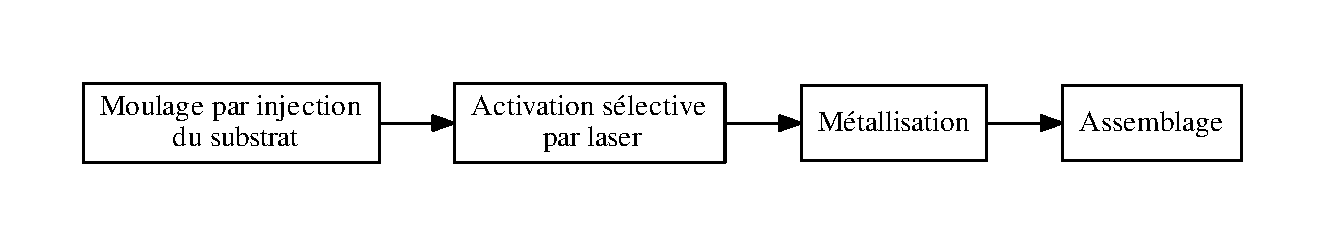
\includegraphics[width=\textwidth]{images/lds_process}
        \caption{Vue d'ensemble du processus \emph{Laser Direct Structuring}}\label{fig:lds-process}
    \end{center}
\end{figure}
Le \gls{lds} est un procédé relativement récent, ayant été introduit sur le marché en 2006.
Par conséquent, c'est une technologie brevetée de LPKF~Lasers~\&~Electronics~AG en Allemagne.
Leur site web\footnote{\url{www.lpkf.com}} est donc une excellente source d'informations pour la conception de pièces utilisant le \gls{lds}.

\subsubsection{Principe de base du procédé}
Le principe général du procédé est visible à la fig.
\ref{fig:lds-process}.
On retrouve donc, dans l'ordre :

\begin{description}
    \item[Injection] La pièce esLa pièce est d'abord moulée par un procédé d'injection standard.
        Le détail de cette étape sort du cadre de ce séminaire.
        On se référera à celui sur l'injection plastique.

    \item[Activation] Le polymère ayant servi pour l'injection de la pièce a préalablement été dopé avec un composant organométallique qui est activé par le laser en suivant le tracé des pistes voulues.
        Une réaction physique décompose alors ce dopant entre partie métallique et partie organique.
    Les lasers utilisés sont typiquement des lasers infra-rouges d'une \item[Métallisation] L'étape de métallisation commence par une étape de nettoyage, afin de faciliter l'accrochage.
        Les pistes sont ensuites construites par dépose de fine couches (environ \SI{5}{\micro\meter}).
        Finalement, un traitement de surface contre l'oxydation est appliqué.
        Ce traitement consiste généralement en une couche de nickel suivi d'une couche d'or, mais des traitements spécifiques, à base d'étain ou d'argent sont également possibles.
    \item[Assemblage] Les composants électriques annexes (boutons, connecteurs, etc\ldots) sont soudés sur le \gls{mid}.
        Pendant le prototypage cette étape est souvent faite à la main, avec un fer à souder.
        Pour la production, si le polymère a une température de fusion suffisament élevée, l'assemblage par \emph{reflow soldering} est possible.

\end{description}

\subsubsection{Métallisation}
L'étape de métallisation est celle qui va déposer les pistes sur le poylmére à proprement parler.
Afin de garantir le bon fonctionnement de cette étape, un rinçage de la pièce entre chaque bains est effectué, ainsi qu'un séchage à chaud après le dernier bain, afin d'enlever toute trace sur la pièce finale.

Le premier bain de cuivre se fait sans électrolyse, vu qu'aucune piste conductrice n'existe pour le moment.
Dans ce bain, du cuivre va croître autour des atomes de métail présent à la surface du polymère et se liera au microcavités résultant de l'activation laser.
L'épaisseur maximum atteignable lors de ce premier bain est de 5 à 8 \si{\micro\meter}.

Dans les applications à fort courants, une grande épaisseur de cuivre est souhaitée.
Pour y parvernir, on peut, après le premier bain, faire une dépose éléctrolytique du cuivre.
Pour cela, il faut que toute les pistes soit connectées entre elles en un point.
Si ce n'était pas le cas, il faudrait connecter les pistes une à une à l'éléctrode, ce qui serait long et donc coûteux.
Le point de connexion est généralement placé sur une partie séparable mécaniquement qui est enlevée après la métallisation.

Une fois ce premier bain terminé, une couche de protection contre l'oxydation est appliquée.
En effet une oxydation de la couche de cuivre ruinerait les proprietés électriques du circuit.
Cette couche est généralement composée d'une couche de nickel suivie d'une couche d'or.
Le rôle de cette dernière est d'empêcher l'oxydation de la couche de cuivre, tandis que la couche de nickel sert à empêcher le cuivre de diffuser dans l'or, ce qui détruirait la protection anti-oxydation.
Avant le traitement anti-oxydant, la pièce est passée dans un bain de palladium \footnote{\emph{A vérifier :} \ce{PdCl2}} afin de catalyser la dépose du nickel.

\subsection{Two-shot molding}
Le two-shot molding est un procédé antérieur au \gls{lds} et qui n'est pas breveté.
Il est essentiellement utilisé dans le milieu de l'injection plastique, pour produire des pièces injectées de différentes couleurs, comme des touches de clavier d'ordinateur.
Cette méthode consiste à d'abord mouler les pistes dans un polymère dopé, puis à ``surmouler'' la forme définitive de la pièce autour (fig. \ref{fig:second-shot}).
Finalement, la pièce est métalisée suivant le même procédé que dans le \gls{lds}, mais le cuivre ne se dépose que sur les parties exposées du polymère dopé (fig. \ref{fig:two-shot-metal}).


\begin{figure}[h]
        \centering
        \begin{subfigure}[t]{0.3\textwidth}
                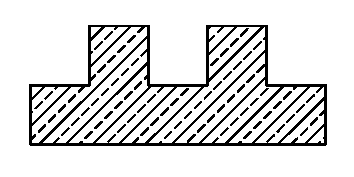
\includegraphics[width=\textwidth]{images/two-shot-example/inner}
                \caption{Injection du polymère dopé.}
                \label{fig:first-shot}
        \end{subfigure}%
        ~ 
        \begin{subfigure}[t]{0.3\textwidth}
                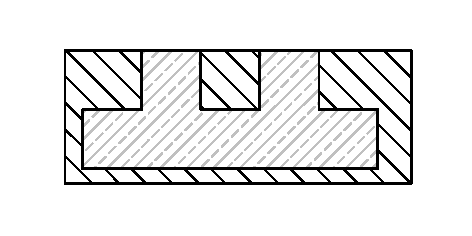
\includegraphics[width=\textwidth]{images/two-shot-example/second_shot}
                \caption{Surmoulage d'un polymère standard.}
                \label{fig:second-shot}
        \end{subfigure}
        ~
        \begin{subfigure}[t]{0.3\textwidth}
                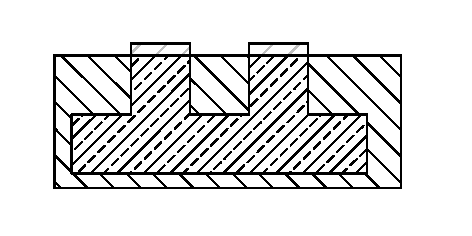
\includegraphics[width=\textwidth]{images/two-shot-example/after_metal}
                \caption{Métallisation.}
                \label{fig:two-shot-metal}
        \end{subfigure}
        \caption{Procédé two-shot}\label{fig:two-shot-process}
\end{figure}




\begin{figure}
        \centering
        \begin{subfigure}[b]{0.4\textwidth}
                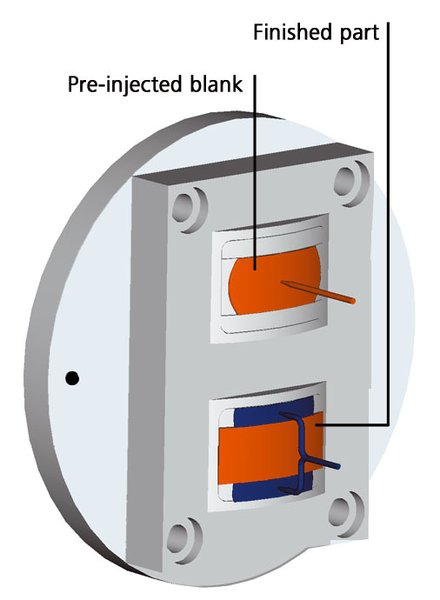
\includegraphics[width=\textwidth]{two-shots-a}
                \caption{Remplissage simultané des moules}
                \label{fig:gull}
        \end{subfigure}%
        ~ 
        \begin{subfigure}[b]{0.4\textwidth}
                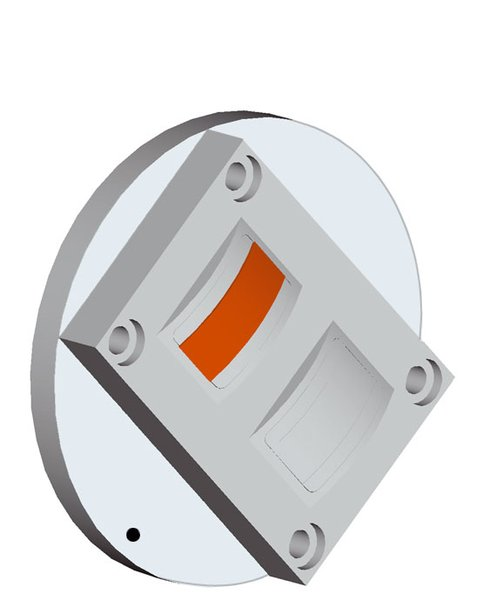
\includegraphics[width=\textwidth]{two-shots-b}
                \caption{Rotation des moules}
                \label{fig:lol}
        \end{subfigure}%
        \caption{Procedé two-shot}\label{fig:animals}

        \floatfoot{Source: \url{http://www.sumitomo-shi-demag.eu/processes/multi-component-technology/rotary-plate.html}}
\end{figure}

\appendix
\listoffigures

\nocite{*} % tells bibtex to include everything
\bibliographystyle{abbrv-fr}
\bibliography{biblio}
\end{document}
